\documentclass[document]{xmgr}
% Jeśli nowe rozdziały mają się zaczynać na stronach
% nieparzystych:
% \documentclass[openright]{xmgr}

%\defaultfontfeatures{Scale=MatchLowercase}
%\setmainfont[Numbers=OldStyle,Ligatures=TeX]{Minion Pro}
%\setsansfont[Numbers=OldStyle,Ligatures=TeX]{Myriad Pro}
% for fontspec version < 2.0
\setmainfont[Numbers=OldStyle,Mapping=tex-text]{Georgia}
\setsansfont[Numbers=OldStyle,Mapping=tex-text]{Times New Roman}
\usepackage{amsmath}
\usepackage{amsfonts}
\usepackage{listings} 
\usepackage{color}
\usepackage{graphicx}
\usepackage{float}
\usepackage[section]{placeins}
\usepackage{tabularx}
\PolyglossiaSetup{polish}{indentfirst=true}
\setmonofont[Scale=0.75]{Monaco}

% Opcjonalnie identyfikator dokumentu
% drukowany tylko z włączoną opcją 'brudnopis':
\wersja   {wersja wstępna [\ymdtoday]}

\author   {Szymon Rękawek}
\nralbumu {206288}
\email    {rekawekszymon@gmail.com}

\title    {Gra Thuego}
\date     {2016}
\miejsce  {Gdańsk}

\opiekun  {prof. UG dr, hab. T. Dzido}

% dodatkowe polecenia
%\renewcommand{\filename}[1]{\texttt{#1}}
\definecolor{stress}{cmyk}{0,1,0.13,0} % RubineRed
\definecolor{topic}{cmyk}{0.98,0.13,0,0.43} % MidnightBlue

%\renewcommand{\lstlistingname}{Metoda}
%\renewcommand{\lstlistlistingname}{Spis metod}



\begin{document}

% streszczenie
\begin{abstract}


\nocite{rampersad2007overlap}

Celem pracy było zaprogramowanie i analiza wyników gry opartej na twierdzeniach Axela Thue, związanej z powtórzeniami oraz nasunięciami wewnątrz ciągu znaków. Głównymi funkcjonalnościami aplikacji jest rozgrywka między dwoma graczami oraz symulacja przeprowadzona przez konkurujące ze sobą algorytmy. 

Powstały dwa warianty aplikacji, pierwszy z~nich napisany został za pomocą silnika \emph{Unity3d}, posiada interfejs graficzny, nie ma jednak innego zastosowania niż poprawianie własnych rekordów. Drugi jest napisany w~jęzku \emph{Java}, bez interfejsu graficznego, w~zamian oferuje funkcjonalność dokonywania testów na serwerze zdalnym i~zawiera wiele opcji konfiguracyjnych, między innymi precyzowanie poziomu rekurencji, którego używają algorytmy.

Przeprowadzone testy wykazały, że algorytmy symulujące graczy działają prawidłowo i~zwiększanie ich poziomu rekurencji skutkuje lepiej podejmowanymi decyzjami. Na podstawie badań ustalona została maksymalna długość rozgrywki przy odpowiedniej taktyce, dla rozgrywek zawierających określoną ilość symboli z~których tworzony jest ciąg.
\end{abstract}

% słowa kluczowe
\keywords{Thue, Java, ciąg, programowanie, Unity3d}

% tytuł i spis treści
\maketitle

% wstęp
\introduction

Tematem niniejszej pracy jest Gra Thuego. Axel Thue był norweskim matematykiem żyjącym w~latach 1863 -- 1922, znanym z~prac z~zakresu kombinatoryki.

Thue pracował nad problemami, powstałymi w~wyniku badań nad sekwencjami symboli. Prace Thue \cite{repetition} opisywały problem, który autor nazwał \emph{nieredukowalnymi słowami}. Poświęca w~nich szczególną uwagę dwu i~trzy literowym przypadkom. W~skrócie wprowadza pojęcie znane obecnie jako \emph{Thue-Morse word} i~pokazuje, że nieskończone \emph{słowa bez nasunięć}, są pochodnymi tej sekwencji. W~swoich pracach definiuje kolejną strukturę, a~mianowicie \emph{nieskończone słowo wolne od kwadratów}, oraz przedstawia sposoby generowania nieskończenie długich słów wolnych zarówno od \emph{kwadratów} jak i~\emph{nasunięć}.

Gra która powstała na podstawie twierdzeń Thuego, w~skrócie polegała będzie na utworzeniu jak najdłuższego ciągu znaków nad określonym z~góry alfabetem. Zależnie od trybu gry, kończyć się będzie ona w~momencie, gdy pojawi się zdefiniowany na początku rodzaj powtórzenia w~tworzonym przez nas, bądź algorytm ciągu. Jednym z~trybów gry jest rozgrywka komputera przeciwko niemu samemu, po jej zakończeniu przedstawiony zostanie czas trwania rozgrywki i~każdego wykonanego ruchu.

Ostatnia część pracy poświęcona jest analizie algorytmów zarówno pod względem czasu ich wykonywania jak i~zdolności do przewidywania ruchów przeciwnika. Badany jest również aspekt tego, ile symboli z~których tworzony jest ciąg, jest potrzebnych na rozegranie dostatecznie długiej rozgrywki, przy możliwie najdoskonalszej taktyce.

\chapter{Opis struktur pozwalających na stworzenie gry}
Zanim przejdziemy do twierdzeń, koniecznym jest wyjaśnienie podstawowych definicji, które w~dalszej części pracy będą wielokrotnie wykorzystywane. Niżej wyjaśnione zostały sposoby generowania nieskończenie długich ciągów składających się z~dwóch symboli, nie zawierających \emph{nasunięć}. Po czym ukazane zostały metody tworzenia nieskończenie długich ciągów na trzech znakach, \emph{wolnych od kwadratów}. Na koniec części teoretycznej przedstawiony został pomysł gry dla dwóch graczy wykorzystujący powyższe własności.


\section{Definicje}


\begin{itemize}
\item \emph{Alfabet} jest skończonym zbiorem symboli lub liter.
\item Słowo \emph{alfabetu} $A$ jest skończoną sekwencją elementów z~$A$. 
\item Długość słowa $\omega$ jest reprezentowana przez $|\omega|$.
\item Puste słowo o~długości $0$ jest reprezentowane przez $\varepsilon$.
\item Czynnik słowa $\omega$ jest słowem $u$, które występuje wewnątrz $\omega$ formie $\omega = xuy$, podczas gdy $x$ oraz $y$ również są słowami tego alfabetu.
\item \emph{Kwadrat} jest słowem w~formie $uu$, gdzie $u$ jest niepuste.
\item Słowo jest \emph{wolne od kwadratów}, jeśli żaden z~jego czynników nie jest \emph{kwadratem}.
\item \emph{Nasunięcie} jest słowem w~formie $xuxux$, gdzie $x$ jest niepuste. Nazwa pojęcia wzięła się z~tego, że $xux$ występuje dwa razy w~$xuxux$. Jako \emph{prefiks} oraz jako \emph{sufiks}, oba wystąpienia mają wspólną część -- centralne $x$, a~więc \emph{nasuwają} się na siebie.
\item Słowo jest \emph{wolne od nasunięć} jeśli żaden z~jego czynników nie nasuwa się na siebie.
\item W~definicji Axela Thue słowo $\omega$ w~alfabecie długości $n$ jest \emph{nieredukowalne}, jeśli jakiekolwiek dwa wystąpienia tego samego słowa jako czynnik wewnątrz $\omega$ są zawsze oddzielone od siebie przez $n-2$ liter. Oznacza to, że nieredukowalne dwuliterowe słowo jest bez \emph{nasunięć} i~nieredukowalne trzyliterowe słowo jest bez \emph{kwadratów}.
\item \emph{Morfizm} -- mapowanie obiektu matematycznego z~jednej struktury w~inną.
\end{itemize}



\section{Thue-Morse word}
Słowo Thue-Morse'a jest nieskończonym ciągiem znaków utworzonym z~dwuliterowego alfabetu,  nie zawierającym ani jednego nasunięcia. Zostało ono nazwane po Thue, który badał jego właściwości w~pracy z~1906 roku \cite{nagell1977selected}, oraz Morsie, który pracował nad nim w~latach 20 XX wieku. Konstrukcja zwana obecnie słowem Thue-Morse'a występuje również o~wiele wcześniej w~korespondencji Prouheta \cite{prouhet} z~Francuską Akademią Nauk w~1851 roku. Prouhet podał więcej ogólnych konstrukcji, uzyskując nie tylko to słowo, ale całą rodzinę słów na większych alfabetach mających inne interesujące właściwości. Słowa te czasami odnoszą się do ogólnych słów Thue-Morse'a lub słów Prouheta. Dla alfabetu $A = \{0, 1\}$ słowo to może wyglądać w następujący sposób:

{\centering $01101001100101101001011001101001\ldots$ \par}

\noindent Jednym ze sposobów generowania słowa Thue-Morse'a jest zastosowanie się do poniższego wzoru.

\begin{tabbing}

\hspace{8em}\= $\mu(a) = ab$,\hspace{7em}\= $\mu(b) = ba$\\
Dla $n \geq 0$:\\
\> $u_n = \mu^n(a)$,\> $v_n = \mu^n(b)$\\
Wtedy:\\
\> $u_0 = a$ \> $v_0 = b$\\
\> $u_1 = ab$ \> $v_1 = ba$\\
\> $u_2 = abba$	 \> $v_2 = baab$\\
\> $u_3 = abbabaab$ \> $v_3 = baababba$\\
Wzór ogólny:\\
\> $u_{n+1} = u_n v_n,$ \> $v_{n+1} = v_n u_n$\\
oraz:\\
\> $u_n = \overline{v}_n,$ \> $v_n = \overline{u}_n$
\end{tabbing}

gdzie $\overline{\omega}$ jest uzyskiwane z~$\omega$ przez zamianę $a$ oraz $b$. Słowa $u_n$ i~$v_n$ są często nazywane \emph{blokami Morsa}. Można łatwo zauważyc że $u_{2n}$ oraz $v_{2n}$ są palindromami oraz to że $u_{2n+1} =  v^{\sim}_{2n+1}$, gdzie $w^{\sim}$ jest odwróceniem $w$. Morfizm $\mu$ może być rozszerzony do nieskończonych słów, które mają dwa stałe punkty:

{\centering 
$t = abbabaabbaababbabaab\ldots = \mu(t)$ \\
$ \overline{t} = baababbaabbabaababba\ldots = \mu(\overline{t})$
\par}

\noindent Przedstawione powyżej słowo $t$ jest sekwencją Thue-Morse'a. Jest wiele innych sposobów na stworzenie tego słowa. Niech $t_n$ będzie $n$-tym symbolem w~$t$, zaczynając od $n =$ 0. Wtedy można pokazać, że:

\[
t_n=
\left \{
\begin{tabular}{ccc}
$a$\ if$\ d_1(n) \equiv 0$ (mod $2$) \\
$b$\ if$\ d_1(n) \equiv 1$ (mod $2$)
\end{tabular}
\right \}
\]

\noindent gdzie $d_1(n)$ jest liczbą bitów równych $1$ w binarnej rozbudowie $bin(n)$ z $n$. Na przykład dla $n \leq 12$ oraz $n \in \mathbb{N}$ generowane jest następujące słowo:

\begin{tabbing}
\centering
$bin(0)$\hspace{1em} \= $= 0,$\hspace{7em} \= $d_1 (0)$\hspace{1em} \= $= 0\ mod\ 2 = 0 \to a$ \\
$bin(1)$ \> $= 1,$ \> $d_1 (1)$ \> $= 1\ mod\ 2 = 1 \to b$\\
$bin(2)$ \> $= 10,$ \> $d_1 (2)$ \> $= 1\ mod\ 2 = 1 \to b$\\
$bin(3)$ \> $= 11,$ \> $d_1 (3)$ \> $= 2\ mod\ 2 = 0 \to a$\\
$bin(4)$ \> $= 100,$ \> $d_1 (4)$ \> $= 1\ mod\ 2 = 1 \to b$\\
$bin(5)$ \> $= 101,$ \> $d_1 (5)$ \> $= 2\ mod\ 2 = 0 \to a$\\
$bin(6)$ \> $= 110,$ \> $d_1 (6)$ \> $= 2\ mod\ 2 = 0 \to a$\\
$bin(7)$ \> $= 111,$ \> $d_1 (7)$ \> $= 3\ mod\ 2 = 1 \to b$\\
$bin(8)$ \> $= 1000,$ \> $d_1 (8)$ \> $= 1\ mod\ 2 = 1 \to b$\\
$bin(9)$ \> $= 1001,$ \> $d_1 (9)$ \> $= 2\ mod\ 2 = 0 \to a$\\
$bin(10)$ \> $= 1010,$	\> $d_1 (10)$ \> $= 2\ mod\ 2 = 0 \to a$\\
$bin(11)$ \> $= 1011,$ 	\> $d_1 (11)$ \> $= 3\ mod\ 2 = 1 \to b$\\
$bin(12)$ \> $= 1100,$ 	\> $d_1 (12)$ \> $= 2\ mod\ 2 = 0 \to a$
\end{tabbing}

{\centering $t = abbabaabbaaba$ \par}

W konsekwencji istnieje skończony automat obliczający wartości $t_n$. Automat ten ma dwa stany końcowe $0$ oraz $1$. Na początku czyta łańcuch znaków $bin(n)$ od lewej do prawej, zaczynając od $n=0$. Ostateczny stan równy jest $0$ lub $1$ i~definiuje czy $t_n$ jest równe $a$ czy $b$. W~skrócie obliczenie jakie wykonuje automat to $d_1(n)\ modulo\ 2$.


\section{Square-free word}
Łatwo można zauważyc, że jedynymi słowami bez kwadratów w~alfabecie $A = \{a, b\}$ są: $a, b, ab, ba, aba, bab$. Istnieje jednak dowolnie długi ciąg znaków wolny od kwadratów, dla słów nad alfabetem trzyliterowym. By stworzyć dowolne słowo wolne od kwadratów, Thue wymyślił następujący algorytm. Mając alfabet $A = \{a, b, c\}$ należy zastąpić każde wystąpienie litery $a$ przez $abac$,  $b$ przez $babc$ oraz $c$ przez $bcac$, jeśli jest poprzedzone przez $a$ lub $acbc$, jeśli jest poprzedzone przez $b$. Zaczynając od litery $a$ otrzymujemy nieskończone słowo które nie zawiera kwadratów.

{\centering $abacbabcabacbcacbabcabacbabcacbcabacbabc...$ \par}

W 1912 roku Axel Thue wymyślił kolejną metodę generowanie nieskończonego słowa bez kwadratów na trzech literach z użyciem następującego morfizmu. 
\begin{itemize}
\item $a \to abcab$
\item $b \to acabcb$
\item $c \to acbcacb$
\end{itemize}


\noindent Po raz kolejny zastępujemy każde wystąpienie z~naszych liter przez zdefiniowane sekwencje. Jest to dość skomplikowana struktura, zsumowana długość łańcuchów wynosi $18$. A. Carpi \cite{carpi} w 1983 roku dowiódł, że morfizm na alfabecie składającym się z~trzech liter tworzący słowa wolne od kwadratów musi mieć długość równą co najmniej $18$.

\section{Thue online}
Praca J. Grytczuka, P. Szafrugi i~M. Zmarza pod tytułem \emph{Online version of theorem of Thue} \cite{thueonline} opisuje grę online bazującą na twierdzeniach Thuego. Podczas rozgrywki dwaj gracze  naprzemiennie wykonując swoje ruchy, tworzą  ciąg bez kwadratów. Celem pierwszego gracza jest jak najszybsze skończenie rozgrywki poprzez utworzenie kwadratu, drugi natomiast musi tego unikać.

Wartym wspomnienia jest uproszczony tryb gry, podczas którego mamy graczy -- Alicję i~Boba, tylko Alicji zależy na tym by uniknąć kwadratów. Rozgrywka polega na tym, że Alicja i~Bob wybierają na przemian symbole z~ustalonego alfabetu $A$, oraz dopisują je na końcu istniejącego ciągu. W~momencie, gdy pojawia się kwadrat $aa$, jego druga część, czyli w~naszym przypadku prawe $a$, zostaje usunięte. Zostało udowodnione w pracy \cite{thueonline2}, że Alicja jest w~stanie stworzyć dowolnie długi ciąg bez kwadratów, nie zważając na ruchy Boba. Powyższe jest jednak możliwe pod warunkiem, że moc zbioru $A$ wynosi conajmniej $8$.

Innym typem gry przedstawionym w~pracy \cite{thueonline} jest \emph{Online Thue Game}. Po raz kolejny gracze wykonują swoje ruchy na przemian. W~swojej rundzie Bob wybiera pozycję $s_i$ w~ciągu $S$, gdzie $i \in \{0, 1,\ldots , n\}$, a $n$ to aktualna długość ciągu. Następnie Alicja wybiera symbol $x$ z alfabetu $A$, który jest wstawiany pomiędzy pozycją $s_{i}$ i $s_{i+1}$, tworząc nowy ciąg $S'=s_1, \ldots, s_i, x, s_{i+1}, \ldots, s_n$. Celem Boba jest wybieranie takich pozycji, by w~sekwencji pojawił się \emph{kwadrat}; Alicja musi wybierać takie symbole by \emph{kwadratu} nie utworzyć. Na przykład, jeśli ustalimy, że alfabet $A = \{0, 1, 2\}$, a~sekwencja $S=0212$, wtedy Bob wybierając pozycję $i=1$,~zmusza Alicję do stworzenia kwadratu w kolejnym ruchu. Każdy z symboli należących do alfabetu $A$, wstawiony na pozycję $i=1$ skutkuje jego utworzeniem: $S^0 = \underline{00}21, S^1=0\underline{1212}, S^2=0\underline{22}12$. W~przypadku gdy Bob obierze dobrą strategię, rozgrywka na $3$ symbolach skończy się na ciągu o~długości $\leq 5$, nie ważne jaką strategię obierze Alicja. Oczywiście im więcej elementów znajduje się w alfabecie $A$, tym więcej ruchów, będzie potrzebował Bob, by wygrać 

Grytczuk, Szafruga i~Zmarza \cite{thueonline} udowodnili, że istnieje strategia dla Alicji gwarantująca jej rozegranie dowolnie długiej gry w~\emph{Online Thue game} na zbiorze 12 symboli. Swoją definicję oparli o~prace A. Kündgena i~M. J. Pelsmajera \cite{first}, oraz J. Baráta i~P. P. Varjú. \cite{second}, na temat niepowtarzalnych kolorowań grafów planarnych. 

\section{Komputerowa implementacja Online Thue Game}

Komputerowa implementacja gry Thuego opiera się na pomyśle gry z~pracy \cite{thueonline}. W~grze dostępne są dwa typy gry, zarówno dla jednego oraz dwóch graczy jak i~komputerowa symulacja, czyli gra komputera przeciwko niemu samemu.

Implementacja gry \emph{Online Thue Game} nazywana będzie \emph{Longest Free Word}. W grze dostępne są dwa typy gry, pierwszy z nich to \emph{Longest Square-Free Word}, a jego zasady są następujące. Na początku gry, gracze ustalają liczbę symboli wchodzących w~skład alfabetu $A$ i~otrzymują swoje role. Jeden z~nich staje się \emph{budowniczym}, drugi \emph{malarzem}. Rola \emph{budowniczego} polega na wybieraniu pozycji w~tworzonym ciągu, na którą wstawiony zostanie wybrany przez \emph{malarza} symbol z~alfabetu $A$. Gra kończy się w~momencie, gdy w~tworzonym przez graczy ciągu pojawi się \emph{kwadrat}. Numer pozycji $i$ podawanej przez \emph{budowniczego} musi spełniać warunek $0 \leq i \leq n$, przy czym $n$ to aktualna ilość elementów w ciągu. Na początku gry sekwencja $S$ zawiera jeden losowy symbol, z alfabetu $A$. Grę rozpoczyna \emph{budowniczy}, a gracze wykonują swoje ruchy na przemian. \emph{Malarz} otrzymuje punkt za każdy wstawiony element, który nie tworzy \emph{kwadratu}. By wyłonić zwycięzcę potrzebne są dwie rundy. Każdy z~graczy musi sprawdzić się w obu rolach. Wygrywa osoba, która zdobyła więcej punktów jako \emph{malarz}.

Gra dostępna jest też dla jednego gracza, rolę przeciwnika otrzymuje wtedy algorytm, który działa według ustawionej w pliku konfiguracyjnym taktyki. Może on zarówno pełnić rolę budowniczego jak i~malarza. Dodatkową możliwością jest przeprowadzenie rozgrywki pomiędzy dwoma algorytmami.

Bliźniaczym typem gry, opierającym się na tych samych zasadach z~niewielką różnicą jest \emph{Longest Overlap-Free Word}. Różnica polega na tym, że malarz w~tworzonym ciągu musi unikać \emph{nasunięcia}. Tutaj podobnie jak w~\emph{Longest Square-Free Word} jest możliwość gry przeciwko algorytmowi, oraz przeprowadzenie rozgrywki dwóch algorytmów.

\chapter{Aplikacja Longest Free Word}
Stworzony przeze mnie program, który powstał na bazie gry \emph{Longest Free Word}, napisany jest w~języku \emph{Java}. Umożliwia on rozgrywkę w~obu wersjach gry, zarówno z~drugim graczem, jak i~z komputerem, oraz jest w~stanie zasymulować rozgrywkę dwóch graczy komputerowych, grających przeciwko sobie z~wybranymi przez użytkownika taktykami. Dodatkową opcją jest uruchomienie obszernego testu, który zasymuluje rozgrywkę komputerowych graczy na wielu kombinacjach poziomów zaawansowania i~alfabetów o różnych rozmiarach. Komunikacja z~grą odbywa się poprzez plik konfiguracyjny -- przed uruchomieniem programu, oraz konsolę -- po jego uruchomieniu. Dzięki użyciu narzędzia automatyzującego budowę aplikacji -- \emph{Maven}, po pobraniu kodu źródłowego, jesteśmy w~stanie uruchomić ją z~poziomu terminala dzięki wprowadzeniu zaledwie dwóch krótkich instrukcji. Okazało się ono niezwykle pomocne podczas przeprowadzania czasochłonnych testów na maszynie zdalnej, której sterowanie odbywało się właśnie poprzez terminal.


\section{Plik konfiguracyjny}
Opcje dostępne wewnątrz pliku konfiguracyjnego to:
\begin{itemize}
\item \emph{gameType} -- wartości, które zmienna akceptuje to \texttt{Square} oraz \mbox{\texttt{Overlap}}. Jest to typ gry, którego zamierzamy użyć i~precyzuje, czy zagramy w~\emph{Longest Square-Free Word} czy \emph{Longest Overlap-Free Word}.
\item \emph{gameMode} -- wartości wpisywane w~tym polu mają wpływ na to, czy gra odbywać się będzie z~drugim człowiekiem - \texttt{humanHuman}, komputerem z~tym warunkiem, że to my jesteśmy budowniczym -- \texttt{humanBuilder}, ponownie z~komputerem, jednak tym razem to on jest budowniczym -- \texttt{pcBuilder}, oraz walka dwóch komputerów -- \texttt{pcPc}.
\item \emph{setPower} -- jest to liczba symboli, do których dostęp będzie miał malarz podczas rozgrywki. Zbiór ten wypełniany jest liczbami  należącymi do zbioru $\{0, 1, ...,n-1\}$.
\item \emph{builderNestingLevel} i~\emph{painterNestingLevel} -- liczba wywołań rekurencyjnej funkcji podczas podejmowania decyzji jako \emph{budowniczy} i~\emph{malarz}. Po ustawieniu tych zmiennych na $0$ algorytmy działają zachłannie. 
\item \emph{maxThinkTime} -- podczas przeprowadzania testów z~udziałem komputerowych graczy, czasami nie chcemy by przeciwnik myślał nad swoim ruchem 17 godzin. Właśnie dlatego została wprowadzona ta opcja konfiguracyjna. Jeśli czas jaki komputer spędził nad wyliczeniem kolejnej pozycji lub symbolu, będzie większy niż ustalona przez nas liczba nanosekund, to rozgrywka zostaje przerwana.
\item \emph{makeOverallTest} -- gdy opcja ta zostanie ustawiona na \texttt{true}, po uruchomieniu aplikacji zostanie przeprowadzony obszerny test, zawierający w~sobie kombinacje rozgrywek algorytmów z~róznymi wartościami zmiennych \emph{builderNestingLevel}, \emph{painterNestingLevel}, \emph{setPower} i \emph{gameType}. Warto wspomnieć, że podczas tego testu opcja \emph{max\-ThinkTime} okazała się niezwykle pomocna.
\item \emph{randomization} -- po ustawieniu tej flagi na \texttt{true}, algorytmy używające rekurencji będą losować swoją decyzję spośród opcji, które wydają im się tak samo atrakcyjne. Dzięki temu komputerowi oponenci zachowują się nieprzewidywalnie i~ciężko jest rozegrać dwie identyczne partie.
\end{itemize}
\newpage
\section{Algorytm szukający powtórzeń wewnątrz ciągu}


\definecolor{dkgreen}{rgb}{0,0.6,0}
\definecolor{gray}{rgb}{0.5,0.5,0.5}
\definecolor{mauve}{rgb}{0.58,0,0.82}


\lstset{frame=tb,
  language=Java,
  aboveskip=3mm,
  belowskip=3mm,
  showstringspaces=false,
  columns=flexible,
  basicstyle={\small\ttfamily},
  numbers=left,
  numberstyle=\tiny\color{black},
  keywordstyle=\color{blue},
  commentstyle=\color{dkgreen},
  stringstyle=\color{mauve},
  breaklines=true,
  breakatwhitespace=true,
  tabsize=3,
}

\lstset{
    inputencoding=utf8x, 
    extendedchars=\true,
    literate=%
    {ą}{{\k{a}}}1
    {Ą}{{\k{A}}}1
    {ę}{{\k{e}}}1
    {Ę}{{\k{E}}}1
    {ó}{{\'o}}1
    {Ó}{{\'O}}1
    {ś}{{\'s}}1
    {Ś}{{\'S}}1
    {ł}{{\l{}}}1
    {Ł}{{\L{}}}1
    {ż}{{\.z}}1
    {Ż}{{\.Z}}1
    {ź}{{\'z}}1
    {Ź}{{\'Z}}1
    {ć}{{\'c}}1
    {Ć}{{\'C}}1
    {ń}{{\'n}}1
    {Ń}{{\'N}}1
}

Metoda \ref{lst:findSquare} ma za zadanie znalezienie kwadratu w~sekwencji, którą reprezentuje przekazana w~parametrze lista obiektów typu \texttt{Integer}. Zmienna \mbox{\texttt{maxSeqSize}} reprezentuje długość najdłuższego podciągu jaki się zmieści w~sekwencji, jeśli dostawimy za nim podciąg o~identycznej długości. Zmienna \mbox{\texttt{minSeqSize}} jest to minimalna długość podciągu, który może składać się na \emph{kwadrat}, naturalnie jest równa $1$. W linii 5 wykonujemy pętlę, wewnątrz, której do metody \texttt{compareSubSeq} przekazywana jest długość podciągu, który składać się będzie na kwadrat, oraz naszą sekwencję. Metoda \texttt{compareSubSeq} zwróci nam lewą część znalezionego \emph{kwadratu}, lub \texttt{null} w~przypadku, gdy taki kwadrat w~sekwencji nie istnieje.

\begin{lstlisting}[caption={Metoda szukająca \emph{kwadratów} wewnątrz listy.},label=lst:findSquare]
List<Integer> findSquare(List<Integer> sequence) {
	List<Integer> squareSeq = null;
	int maxSeqSize = sequence.size()/2;
	int minSeqSize = 1;
	for(int subSeqSize=minSeqSize; subSeqSize<=maxSeqSize;subSeqSize++) {
		squareSeq = compareSubSeq(subSeqSize, sequence);
		if(squareSeq != null) {
			return squareSeq;
		}
	}
	return null;
}
\end{lstlisting}

Metoda \ref{lst:compareSubSeq}, porównuje sąsiadujące ze sobą podciągi i sprawdza czy są takie same. Zmienne \texttt{left} i~\texttt{right} są to podciągi, które reprezentują lewą i~prawą część kwadratu $aa$. Zmienna \texttt{comparesFitInSequence} jest to ilość porównań jaka zmieści się wewnątrz naszej sekwencji. Dla przykładu, gdy nasz ciąg, jest reprezentowany przez $S=01201020$, a~wcześniej sprecyzowana długość podciągu, składającego się na kwadrat wynosi $2$, to wartość jaka zostanie przypisana do zmiennej \mbox{\texttt{comparesFitInSequence}} wyniesie $(8 + 1) - (2 * 2)=5$, ponieważ możliwe są następujące porównania: $\underline{0120}1020$, $0\underline{1201}020$, $01\underline{2010}20$, $012\underline{0102}0$, $0120\underline{1020}$
W pętli znajdującej się w~linii 5 do lis\-ty \texttt{left} oraz \mbox{\texttt{right}} dodawane są podciągi odpowiedniej długości, natomiast w~linii 10 następuje sprawdzenie czy podciągi są identyczne. Jeśli tak, oznacza to, że w~naszej sekwencji, rozpoczynając od indeksu $i$ występuje kwadrat długości $2 * \texttt{subSeqSize}$. Jeśli listy są różne to w~linii 13 następuje ich wyczyszczenie, po to by pętla mogła porównać dwa kolejne podciągi.

\begin{lstlisting}[caption={Metoda pomocnicza przy szukaniu \emph{kwadratów} wewnątrz listy.},label=lst:compareSubSeq]
Subsequence compareSubSeq(int subSeqSize, List<Integer> sequence) {
	List<Integer> left = new ArrayList<>();
	List<Integer> right = new ArrayList<>();
	int comparesFitInSequence = (sequence.size() + 1) - (subSeqSize*2) ;
	for(int i=0; i<comparesFitInSequence; i++) {
		for(int j =0;j<subSeqSize;j++) {
			left.add(sequence.get(i+j));
			right.add(sequence.get(i+j+subSeqSize));
		}
		if(listsAreEqual(left, right)) {
			return new Subsequence(left, i, subSeqSize);
		}
		left.clear();
		right.clear();
	}
	return null;
}
\end{lstlisting}

Działanie algorytmu szukającego \emph{kwadratów} zilustrowane zostało na rysunku \ref{fig:squareFinding}. Alfabet symboli składa się w tym przypadku ze zbioru liter $\{a, b, c\}$, zamiast ze zbioru cyfr, po to by rysunek był bardziej czytelny. Ciąg w którym szukamy \emph{kwadratu} to $S=abcbc$, kolumny na rysunku reprezentują pierwszą i~drugą iterację pętli z metody \ref{lst:findSquare}. Wiersze natomiast odpowiadają iteracjom pętli z metody \ref{lst:compareSubSeq}. Kolorowe symbole na które wskazują strzałki mówią nam o tym, które podciągi są ze sobą porównywane. Jak widzimy w ciągu nie ma \emph{kwadratu} składającego się z podciągów długości $1$. Algorytm przechodzi więc do drugiej iteracji i~porównuje ze sobą podciągi długości $2$. W drugim wierszu, czyli drugiej iteracji pętli z~metody \ref{lst:compareSubSeq} zostały znalezione dwa takie same podciągi,  w tym momencie algorytm kończy swoją pracę i~zwraca podciąg $bc$.

\begin{figure}[tbh]
    \centering
    \caption{Działanie algorytmu szukającego \emph{kwadratów}.}
    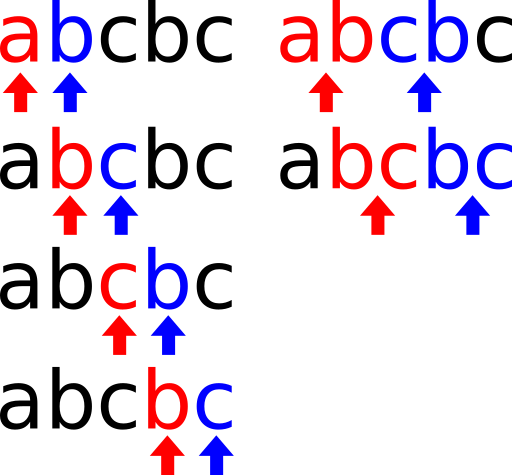
\includegraphics[width = 0.8\textwidth]{images/squareFinding}
    \label{fig:squareFinding}
\end{figure}

Dla typu gry \emph{Longest Overlap-Free Word} potrzebny jest osobny algorytm wyszukujący  \emph{nasunięcia}. Metoda \ref{lst:findOverlap}, działa w~sposób analogiczny do metody \ref{lst:findSquare}. Różnice to inne wartości zmiennych \texttt{maxSeqSize} i~\texttt{minSeqSize} oraz metoda porównująca podciągi wywoływana w~pętli.

Do zmiennej \texttt{maxSeqSize} przypisywana jest liczba o~jeden większa niż długość sekwencji, ponieważ szukamy nasunięcia, a~więc podciągi będą ze sobą dzieliły jeden znak. Wobec tego dla ciągu $S = 0120121$, najdłuższy porównywany ciąg będzie długości $4$, ponieważ w~ostatniej iteracji pętli będziemy ze sobą porównywali podciągi $0120$ oraz $0121$, które dzielą ze sobą symbol $0$. Wartość zmiennej \texttt{minSeqSize} wynosi $3$, ponieważ jest to warunkiem stworzenia nasunięcia.

\begin{lstlisting}[caption={Metoda szukająca \emph{nasunięć} wewnątrz listy.},label=lst:findOverlap]
Subsequence findOverlap(List<Integer> sequence) {
	Subsequence repeatedSequence = null;
	int maxSeqSize = (sequence.size()/2)+1;
	int minSeqSize = 3;
	for(int subSeqSize=minSeqSize; subSeqSize<=maxSeqSize; subSeqSize++) {
		repeatedSequence = compareSubSeqOverlap(subSeqSize, sequence);
		if(repeatedSequence != null) {
			return repeatedSequence;
		}
	}
	return null;
}
\end{lstlisting}

Metoda \ref{lst:compareSubSeqOverlap} działa na tej samej zasadzie co metoda \ref{lst:compareSubSeq}. Różni się tutaj wartość zmiennej \texttt{comparesFitInSequence}, jest ona większa o~$1$, z~takiego samego powodu, co zmienna \texttt{maxSeqSize} z~metody \ref{lst:findOverlap}. Inny jest również podciąg zapisywany do zmiennej \mbox{\texttt{right}}, w~pętli w~6 linii. Pierwszy indeks owego podciągu jest równy indeksowi ostatniego elementu lewego podciągu, po to by stworzyć nasunięcie.

\begin{lstlisting}[caption={Metoda pomocnicza przy szukaniu \emph{nasunięć} wewnątrz listy.},label=lst:compareSubSeqOverlap]
Subsequence compareSubSeqOverlap(int subSeqSize, List<Integer> sequence) {
	List<Integer> left = new ArrayList<>();
	List<Integer> right = new ArrayList<>();
	int comparesFitInSequence = (sequence.size() + 2) - (subSeqSize*2);
	for(int i=0; i<comparesFitInSequence; i++) {
		for(int j =0;j<subSeqSize;j++) {
			left.add(sequence.get(i+j));
			right.add(sequence.get(i+j+subSeqSize-1));
		}
		if(listsAreEqual(left, right)) {
			return new Subsequence(left, i, subSeqSize);
		}
		left.clear();
		right.clear();
	}
	return null;
} 
\end{lstlisting}

Działanie algorytmu ilustruje rysunek \ref{fig:overlapFinding}. Tutaj również alfabet symboli składa się ze zbioru liter $\{a, b, c\}$, by poprawić czytelność rysunku. Ciąg wewnątrz, którego szukamy \emph{nasunięcia} to $S=abaabaa$. Kolumny reprezentują pierwszą i~drugą iteracjię pętli z~metody \ref{lst:findOverlap}, wiersze odpowiadają iteracjom pętli z~metody \ref{lst:compareSubSeqOverlap}. Czerwone i niebieskie symbole wskazywane przez strzałki to porównywane podciągi, różowy symbol to element wspólny obu podciągów. \emph{Nasunięcie} znaleziono w drugiej iteracji metody \ref{lst:findOverlap}, przy pierwszym porównaniu -- podciągi $abaa$ dzielą ze sobą symbol $a$. Po znalezieniu \emph{nasunięcia} algorytm zwraca podciąg $abaa$.

\begin{figure}[tbh]
    \centering
    \caption{Działanie algorytmu szukającego \emph{nasunięć}.}
    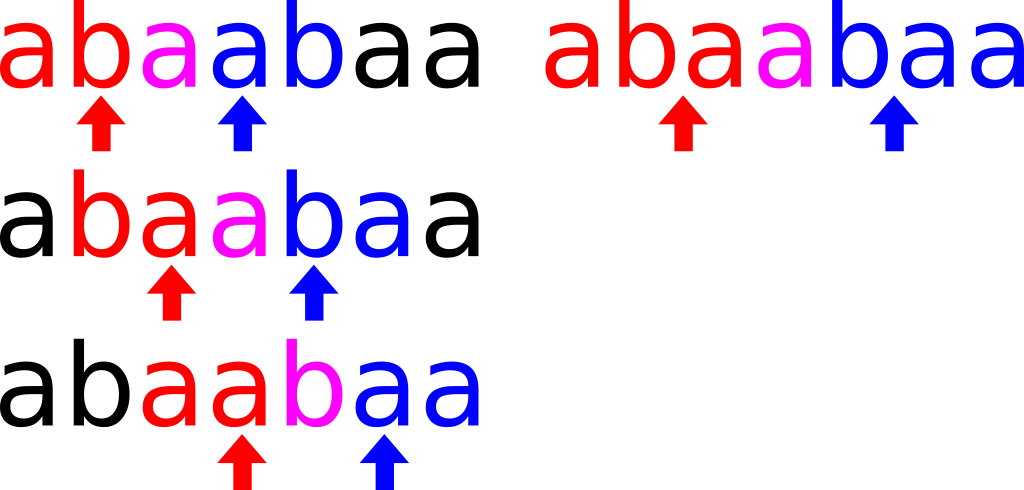
\includegraphics[width = 0.8\textwidth]{images/overlapFinding}
    \label{fig:overlapFinding}
\end{figure}

\section{Komunikacja z~użytkownikiem}
Plik konfiguracyjny nie jest wystarczającym środkiem komunikacji z~aplikacją. W~związku z~tym, po uruchomieniu programu mamy dostęp do konsoli, która służy do wyświetlania jak i~wprowadzania treści.

Po uruchomieniu aplikacji na ekranie wypisywane są najważniejsze op\-cje konfiguracyjne, takie jak poziom budowniczego, poziom malarza oraz lista dostępnych symboli. Jeśli uruchomiliśmy grę w~trybie \texttt{humanHuman}, to aplikacja w~pierwszej kolejności poprosi nas o~indeks. Po wpisaniu indeksu należącego do zbioru \mbox{$\{0, 1, \ldots,n\}$}, program zażąda podania symbolu, powinien on należeć do naszego alfabetu, czyli symbol musi należeć do zbioru \mbox{$\{0, 1, \ldots, setPower-1\}$}. W~momencie gdy podaliśmy prawidłowe wartości na ekran konsoli wyświetlany zostaje ciąg $S'$, który został utworzony poprzez dodanie do istniejącego ciągu odpowiedniego symbolu. Jeśli w~ciągu $S'$ pojawi się kwadrat, wyświetlony zostanie czas rozgrywki, ilość ruchów jaka została do tej pory wykonana oraz indeksy wraz z~symbolami, wspomnianego powtórzenia. Przykład rozgrywki przedstawia kod \ref{lst:gameExample}.

\begin{lstlisting}[caption={Rozgrywka dwóch graczy wypisana w konsoli.},label=lst:gameExample]
#> W grze dostepne sa nastepujace liczby: 
0
1
2
 0: { 0 }  1: {   } 
## =============================================================== ##
#> Podaj indeks: 
1
#> Podaj liczbe: 
2
 0: { 0 }  1: { 2 }  2: {   } 
## =============================================================== ##
#> Podaj indeks: 
1
#> Podaj liczbe: 
1
 0: { 0 }  1: { 1 }  2: { 2 }  3: {   } 
## =============================================================== ##
#> Podaj indeks: 
3
#> Podaj liczbe: 
1
 0: { 0 }  1: { 1 }  2: { 2 }  3: { 1 }  4: {   } 
## =============================================================== ##
#> Podaj indeks: 
4
#> Podaj liczbe: 
2
 0: { 0 }  1: { 1 }  2: { 2 }  3: { 1 }  4: { 2 }  5: {   } 
## =============================================================== ##

#> Znaleziono kwadrat:  
 1: { 1 }  2: { 2 }  <->  3: { 1 }  4: { 2 } 

## =============================================================== ##

#> Rozrgrywka trwala 5 ruchow i 20.339 sekund.
\end{lstlisting}
Jeśli uruchomimy rozgrywkę z~komputerem, obok wybranego indeksu lub symbolu pojawia się również czas jaki był mu potrzebny na podjęcie decyzji(kod \ref{lst:pcPcExample}).

\begin{lstlisting}[caption={Sposób wyświetlania podjętych decyzji algorytmu.},label=lst:pcPcExample]
#> Komputer wybral indeks: 1 	| Czas trwania obliczen: 24.127 s
#> Komputer wybral liczbe: 4 	| Czas trwania obliczen: 0.012 s
\end{lstlisting}
\noindent By ułatwić późniejszą analizę wszystkie informacje zawarte w~konsoli, zapisywane są do nowo utworzonego pliku w~katalogu \underline{output}.

\section{Zachłanny algorytm wyszukiwania symbolu}
Jak zostało wcześniej wspomniane można sterować rodzajami taktyk komputerowych graczy za pomocą zmiennych konfiguracyjnych. Jeśli zmienną \emph{painterNestingLevel} ustawimy na $0$, algorytm \emph{malarza} działał będzie zachłannie, wybierając opcje, która jest najatrakcyjniejsza w~danym momencie, nie zważając na to, co może wydarzyć się w~kolejnej turze. Zasada działania zachłannego algorytmu \emph{malarza} zapisana jest w metodzie \ref{lst:findRightColorGreedy}. Definicja metody mówi nam o trzech parametrach jakie są do niej przekazywane:
\begin{itemize}
\item \texttt{sequence} -- utworzony wcześniej ciąg,
\item \texttt{index} -- indeks wybrany przez budowniczoego,
\item \texttt{power} -- moc alfabetu.
\end{itemize}
Na alfabet, z którego może korzystać \emph{malarz} składają się liczby należące do zbioru $\{0, 1, ..., power-1\}$. W~2 linii metody rozpoczyna się pętla, która iteruje po wszystkich dostępnych symbolach. W~kolejnej linii symbol dodawany jest do naszego ciągu na podanej pozycji. Metoda \texttt{pickProperFind} z~warunku \texttt{if} zależnie od typu gry wywołuje wcześniej opisane metody \texttt{findSquare} lub \texttt{findOverlap}. Jeśli warunek \texttt{if} zostanie spełniony oznacza to, że po dodaniu aktualnego symbolu na danej pozycji nie powoduje stworzenia \emph{kwadratu}/\emph{nasunięcia}, algorytm zatem usuwa dodany element z~ciągu i~zwraca go w~linii 6. Jeżeli  okaże się jednak, że dodany symbol tworzy powtórzenie w~ciągu, zostaje on również usunięty, a~pętla zaczyna się od początku. Metoda zwraca wartość $-1$, jeśli okaże się, że żaden z~symboli nie jest w~stanie stworzyć ciągu wolnego od \emph{kwadratów}/\emph{nasunięć}.

\begin{lstlisting}[caption={Metoda zachłannie szukająca symbolu.},label=lst:findRightColorGreedy]
int findRightColorGreedy(List<Integer> sequence, int index, int power) {
		for(int symbol=0;symbol<power; symbol++) {
			sequence.add(index, symbol);
			if(pickProperFind(sequence) == null) {
				sequence.remove(index);
				return symbol;
			} else {
				sequence.remove(index);
			}
		}
		return -1;
	}
\end{lstlisting}

\section{Zachłanny algorytm wyszukiwania indeksu}
By można było przeprowadzić symulację gry, należy wprowadzić również algorytm \emph{budowniczego}, starający się znaleźć najmniej atrakcyjny indeks dla \emph{malarza}. Zachłanny algorytm realizujący to zadanie znajduje się w metodzie \ref{lst:findRightIndexGreedy}. Metoda jako parametry, otrzymuje stworzony wcześniej ciąg oraz moc zbioru symboli. Zmienna \texttt{winner} ustawiona początkowo na $-1$, reprezentuje indeks, który zostanie zwrócony jako ten, pod którym jest najmniejsza dowolność wyboru symboli, bez tworzenia powtórzeń. Metoda iteruje po każdym indeksie ciągu i~zapisuje do listy symbole, po których wstawieniu w~dane miejsce nie utworzy się \emph{kwadrat}/\emph{nasunięcie}. Następnie w~warunku \texttt{if} z~6 linii sprawdzane jest, czy aktualna lista symboli jest mniejsza lub równa, niż ta zarejestrowana wcześniej. Jeśli tak, do zmiennej \texttt{winner} zapisany zostaje aktualny indeks.

\begin{lstlisting}[caption={Metoda zachłannie szukająca indeksu.},label=lst:findRightIndexGreedy]
int findRightIndexGreedy(List<Integer> sequence, int power) {
	int winner = -1;
	int smallestSymbolSize = power;
	for (int i =0;i<sequence.size()+1;i++) {
		List<Integer> symbols = getFitableColorList(sequence, i);
		if (symbols.size() <= smallestSymbolSize) {
			smallestSymbolSize = symbols.size();
			winner = i;
		}
	}
	return winner;
}
\end{lstlisting}

\section{Algorytm wyszukiwania symbolu z~zagnieżdżeniami}
Algorytm zachłanny nie jest wystarczająco sprytny, żeby przeciwstawić się człowiekowi mającemu odrobinę doświadczenia w~\emph{Longest Free Word}. Wobec tego powstał algorytm nie działający zachłannie, lecz starający się przewidzieć, jakie konsekwencje w~kolejnych turach może nieść ze sobą dany wybór.

Algorytm z metody rekurencyjnie wyszukujący symbolu wprowadza pojęcie punktacji. Podczas jego działania, dla możliwych wyborów nadawane są punkty. Im więcej punktów uzyska dany symbol, tym atrakcyjniejszym staje się on wyborem. Algorytm sprawdza jakie symbole można dodać na predefiniowanej pozycji, następnie iterując w~pętli, dodaje każdy z~symboli i~sprawdza, ile możliwości będzie miał w~kolejnej lub kolejnych turach, biorąc pod uwagę wszystkie dostępne pozycje. Każda dodatkowa możliwość to dodatkowy punkt dla wybranego koloru. Sam algorytm składa się z~dwóch metod głównych \mbox{\texttt{findRightColorPredicting}} (\ref{lst:findRightColorPredicting}) oraz \texttt{simulation} (\ref{lst:simulation}).

Na początku algorytm inicjalizuje listy \texttt{scoreList} oraz \texttt{symbolList}. Tę pierwszą tyloma zerami ile jest w~grze dostępnych symboli, drugą natomiast symbolami, jakie możemy wstawić na zdefiniowanej przez \emph{budowniczego} pozycji. Linia 4 rozpoczyna pętlę, która iterując po liście \texttt{symbolList}, dodaje jej element, wywołuje metodę \texttt{simulation}, przekazując utworzony \emph{ciąg}, dodany \emph{symbol}, \texttt{scoreList} oraz \emph{poziom zagnieżdżenia malarza}, po czym usuwa dodany \emph{symbol} sprawiając, że ciąg pozostaje bez zmian. Na końcu zwraca element, który miał największą liczbę punktów. Jeśli kilka symboli otrzymało ich tyle samo, a~flaga \texttt{randomization} ma wartość \texttt{true} program wybiera losowy z~nich. Dzięki temu w~grze występuje przypadkowość, oraz jest mała szansa na powtórzenie dwóch identycznych rozgrywek przy odpowiednio długim ciągu.

\begin{lstlisting}[caption={Metoda szukająca symbolu, wykorzystująca rekurencję.},label=lst:findRightColorPredicting]
int findRightColorPredicting(List<Integer> sequence, int index) {
	List<Integer> scoreList = initScoreList(power);
	List<Integer> symbolList = getFitableSymbolList(sequence, index);
	for(int symbol: symbolList) {
		sequence.add(index, symbol);
		simulation(sequence, symbol, scoreList, painterNestingLevel);
		sequence.remove(index);
	}
	return getRandomFromScoreList(scoreList);
}
\end{lstlisting}

Wewnątrz metody \texttt{simulation} nadawane są punkty oraz za pomocą rekurencji wykonywana jest symulacja kolejnych iteracji gry. Na początku dekrementowana zostaje zmienna \texttt{invokes} mówiąca o tym, na ile poziomów rekurencji algorytm ma się jeszcze zagłębić. Oznacza to, że jeśli przekazana zmienna \texttt{invokes} ustawiona jest na $1$,~to metoda \texttt{simulation} zostanie wywołana tylko raz. Pętla w~3 linii iteruje po pozycjach, na których możliwe jest dodanie symbolu. W~4 linii do listy zapisywane są symbole, które można wstawić na aktualnej pozycji, nie powodując \emph{kwadratu/nasunięcia}. Metoda \texttt{updateScoreList} zwiększa ilość punktów symbolu przekazanemu z~poprzedniej metody. Ilość punktów jest równa liczbie elementów, zmiennej \texttt{symbolList}. Pętla w~6 linii iterując po liście pasujących symboli, dodaje element, następnie pod warunkiem, że \mbox{\texttt{invokes}} jest większe od $0$, wywołuje samą siebie ze zmodyfikowanym ciągiem, tym samym indeksem, który został przekazany na początku, listą punktową oraz pozostałą liczbą wywołań. Na końcu pętli element zostaje usunięty, po to, by ciąg wrócił do pierwotnego stanu.

\begin{lstlisting}[caption={Metoda rekurencyjnie wykonująca symulacje kolejnych ruchów.},label=lst:simulation]
void simulation(List<Integer> sequence, int indexInScoreList, List<Integer> scoreList, int invokes) {
	invokes--;
	for(int j=0;j<sequence.size()+1;j++) {
		List<Integer> symbolList = getFitableSymbolList(sequence, j);
		updateScoreList(scoreList, indexInScoreList, symbolList.size());
		for(int symbol: symbolList) {
			sequence.add(j, symbol);
			if(invokes > 0) {
				simulation(sequence, indexInScoreList, scoreList, invokes);
			}
			sequence.remove(j);
		}
	}
}
\end{lstlisting}

Działanie algorytmu przedstawione zostało na rysunku \ref{fig:nestingPainter}. Po raz kolejny w celu zwiększenia przejrzystości rysunku alfabet symboli składa się ze zbioru liter $\{a, b, c\}$, a~nie z~liczb jak ma to miejsce podczas zwykłej rozgrywki. Mamy ciąg $S = ab$, \emph{budowniczy} wybrał indeks $2$, zatem \emph{malarz} wybiera symbol jaki zostanie wstawiony za literką $b$. Typ gry to \emph{Longest Square-Free Word}. Wstawienie symbolu $b$, stworzyłoby kwadrat, dlatego algorytm rozważa literki $a$ oraz $c$. Zmienna $n$ jest to poziom rekurencji, natomiast liczby przy pasujących symbolach oznaczają punkty, jakie zostają przypisane symbolowi $a$ lub $c$. 

Już przy pierwszym poziomie rekurencji widać, że literka $c$ jest atrakcyjniejsza, ponieważ wstawienie jej zapewnia \emph{malarzowi} $6$ możliwości w~kolejnych rundach, podczas gdy literka $a$ osiągnęła wynik $4$. Jednak sprawdzenie jednego ruchu do przodu nie zawsze jest wystarczające i~zdarza się, że z~pozoru nieatrakcyjny symbol w~perspektywie kolejnych tur jest najlepszą opcją.
\begin{figure}[tbh]
    \centering
    \caption{Działanie algorytmu rekurencyjnego \emph{malarza}.}
    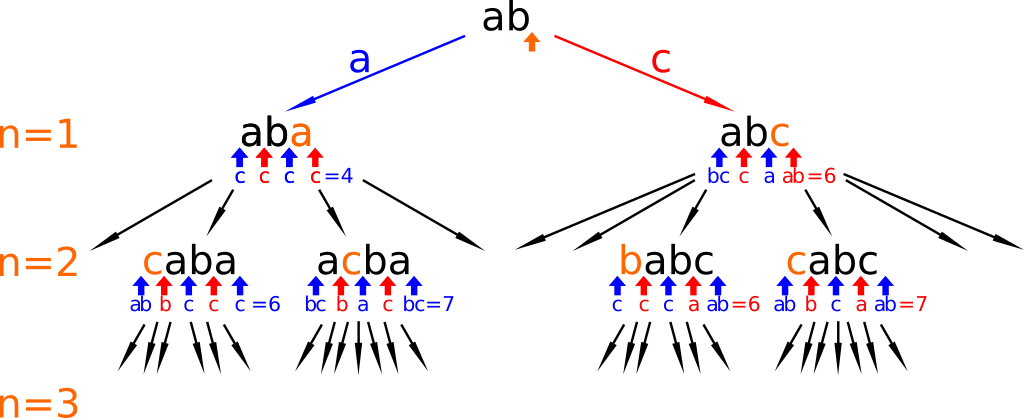
\includegraphics[width = \textwidth]{images/nestingPainter}
    \label{fig:nestingPainter}
\end{figure}



\section{Algorytm wyszukiwania indeksu z~zagnieżdżeniami}
Sposób działania algorytmu rekurencyjnego szukającego indeksu, który ma największą szansę na stworzenie powtórzenia, działa na podobnej zasadzie, co algorytm wyszukiwania symbolu. Różnica polega na tym, że w~jego pierwszej części, ustalamy punktację iterując po wszystkich dostępnych pozycjach, zamiast sprawdzać ją dla jednej ustalonej przez przeciwnika, oraz punkty nadawane zostają pozycjom i~zwracamy tą, która uzyska ich najmniej. Druga część algorytmu czyli metoda \texttt{simulation} (\ref{lst:simulation}) pozostaje bez zmian.

Na początku metody \ref{lst:findRightIndex} zainicjalizowana zostaje zmienna \texttt{scoreList}. Do listy dodane zostają zera w~ilości odpowiadającej długości ciągu plus jeden, bo właśnie na tylu pozycjach możemy dodać nowy element. W~3 linii iterujemy po każdej dostępnej pozycji, natomiast od 4 linii mamy już wszystko to co w~algorytmie szukającym symbolu. Na końcu metody zwracana zostaje pozycja, która uzyskała najmniej punktów, czyli będzie najmniej atrakcyjna dla \emph{malarza}. Tak jak poprzednio jeśli istnieje więcej niż jedna pozycją z~minimalną wartością, a~flaga \texttt{randomization} ustawiona jest na \texttt{true}, to element jest wybierany losowo.

\begin{lstlisting}[caption={Metoda szukająca pozycji, wykorzystująca rekurencję.},label=lst:findRightIndex]
int findRightIndex(List<Integer> sequence) {
	List<Integer> scoreList = initScoreList(sequence.size() + 1);
	for (int i = 0; i<sequence.size() + 1; i++) {
		List<Integer> symbols = getFitableSymbolList(sequence, i);
		for (int symbol : symbols) {
			sequence.add(i, symbol);
			simulation(sequence, i, predictList, builderNestingLevel);
			sequence.remove(i);
		}
	}
	return getRandomMinFromPredict(scoreList);
}
\end{lstlisting}

\section{Longest square free word z interfejsem graficznym}
Napisana została przeze mnie również druga wersja gry. Użytkownik nie korzysta w~niej z~konsoli, lecz z~graficznego interfejsu. W~tej odmianie gracz za pomocą trzech kolorów ma stworzyć jak najdłuższy ciąg bez \emph{kwadratów}. Czynności jakie należy wykonywać podczas rozgrywki to wybranie miejsca, w~które zostanie wstawiony element oraz wybranie jego koloru. Jeśli w~tworzonym ciągu pojawi się \emph{kwadrat} rozgrywka zostaje przerwana i~na ekranie zostają podświetlone powtórzenia składające się na \emph{kwadrat}. Program zapisuje również najwyższy wynik, który jest równy długości utworzonego ciągu. Algorytm szukający \emph{kwadratów} nie różni się w~żaden sposób od tego z~podstawowej wersji gry. Wygląd aplikacji został przedstawiony na rysunku \ref{fig:thueMobile}.

\begin{figure}[tbh]
    \centering
    \caption{\emph{Longest Free Word} z interfejsem graficznym.}
    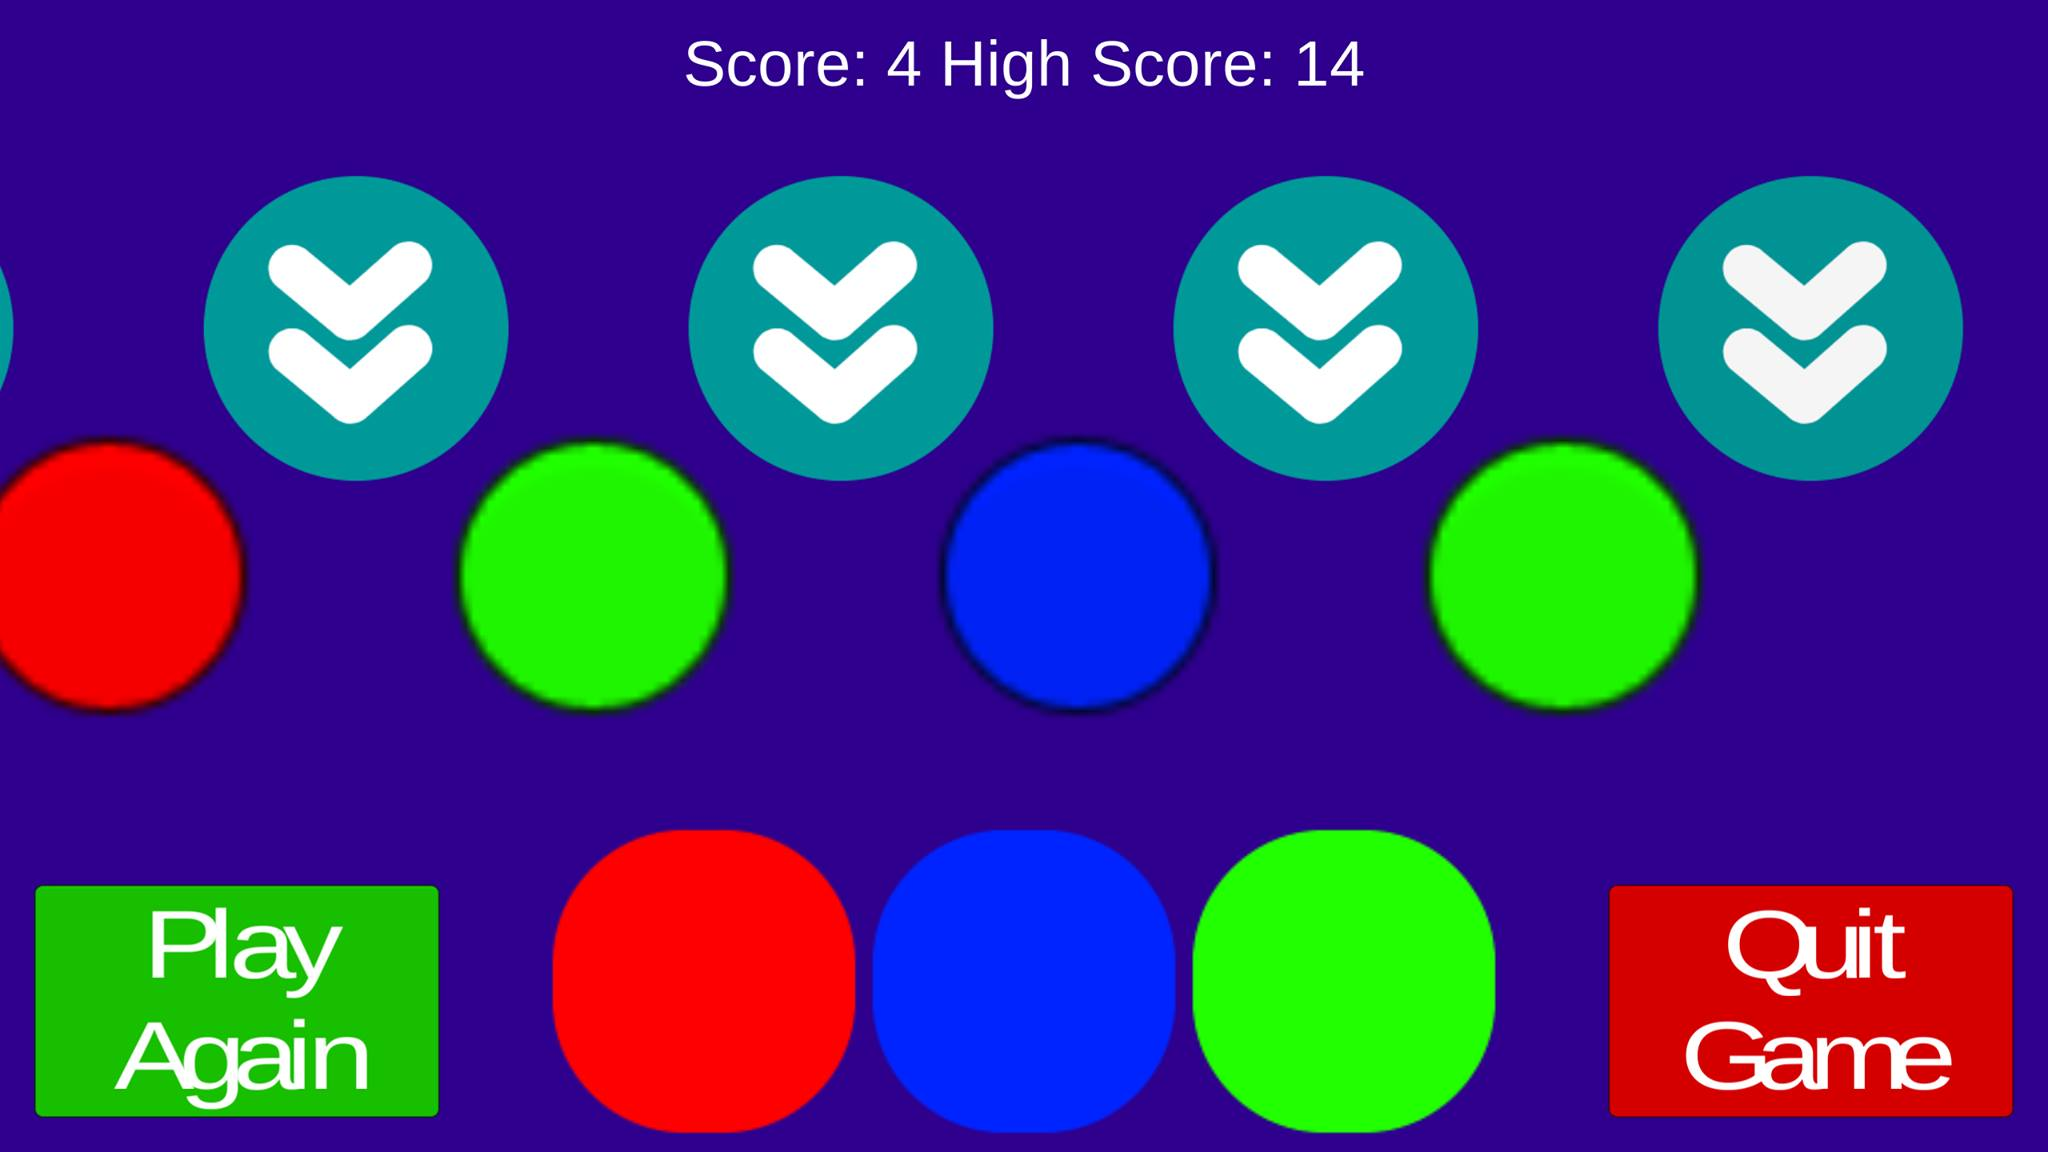
\includegraphics[width = 0.9\textwidth]{images/thueMobile}
    \label{fig:thueMobile}
\end{figure}

Aplikacja została napisana na popularnym silniku do tworzenia gier -- \emph{Unity3d}. Pozwala on kompilować kod programu do plików wykonywalnych, które mogą być uruchamiane w~przeglądarkach, na komputerach osobistych, konsolach i~telefonach komórkowych. W~tym przypadku pod uwagę brane były głównie telefony komórkowe, o~czym może świadczyć wielkość przycisków i~mała ilość wyświetlonych szczegółów.


\chapter{Analiza symulowanych potyczek} 
Dobrym sposobem by poznać aplikację jest jej uruchomienie. Jeszcze lepszym, przeprowadzenie jej analizy oraz zobrazowanie wyników za pomocą wykresów i~tabel. Rozdział ten poświęcony jest badaniu działania aplikacji \emph{Longest Free Word}. Badania skupiają się na wariancie aplikacji opierającym się na tworzeniu ciągu bez \emph{kwadratów}, a~flaga \emph{randomization} ustawiona została na \texttt{true}. Wszystkie testy uruchomione były na zdalnym serwerze, stworzonym za pośrednictwem serwisu \emph{digitalocean.com}. Podzespoły maszyny to system operacyjny Ubuntu 15.10, procesor 2,6 Ghz Intel Core i7, pamięć ram 16 GB 1600 MHz DDR3 i~dysk SSD.



\section{Ilość symboli potrzebna na rozegranie partii}
Długość gry zależna jest od dwóch czynników. Ustawionego poziomu zagnieżdżenia i~ilości dostępnych symboli. Thue w~swoim twierdzeniu \cite{repetition}, udowodnił, że jesteśmy w~stanie stworzyć nieskończenie długi ciąg bez \emph{kwadratów}, mając do dyspozycji alfabet składający się z $3$ symboli. Sytuacja zmienia się, gdy ciąg tworzony jest przez dwóch graczy, z~których jeden stara się utworzyć \emph{kwadrat}. Jeśli  rolę \emph{budowniczego} pełnił będzie zachłanny algorytm, a rolę \emph{malarza} przejmie algorytm wykorzystujący siedmiopoziomową rekurencję, to przy takim alfabecie, rozgrywka i tak zawsze trwała będzie maksymalnie $5$ ruchów. 

Dla alfabetu składającego się z $4$ symboli, algorytmy również nie są w~stanie rozegrać zbyt długiej partii. Przy rozgrywce, w~której udział bierze zachłanny algorytm pełniący rolę \emph{budowniczego}, niezależnie taktyki wybranej przez algorytm \emph{malarza}, rozgrywka zakończy się maksymalnie po $10$ ruchu.

Tabela \ref{fig:maxGameLength}, przedstawia jakim wynikiem kończy się każda z~rozgrywek po przypisaniu odpowiednich wartości zmiennym konfiguracyjnym \emph{setPower}, \emph{builderNestingLevel} i~\emph{painterNestingLevel}. Wartym zauważenia jest, że przy alfabecie o~mocy $4$, zachłanny algorytm pełniący rolę \emph{malarza} (\emph{painterNestingLevel} $=0$), jest w stanie rozegrać partię na $10$ ruchów, a~rozgrywka algorytmów rekurencyjnych \mbox{(\emph{painterNestingLevel} $\geq 1$)}, kończy się po $7$ ruchach. Dowodzi to tego, że taktyka wykorzystująca rekurencje nie jest doskonała i~nie zawsze jest najlepszą opcją. Pozostałe warianty nie zostały przedstawione, gdyż rozgrywka w~ich przypadku nie skutkowała stałym wynikiem. Oznacza to, że taktyka \emph{budowniczego} nie była wystarczająco dobra by za każdym razem pokonać \emph{malarza} w~takiej samej ilości ruchów.

\begin{table}[tbh]
    \centering
	\caption{Maksymalna ilość ruchów w stosunku do ilości dostępnych symboli.}
	\begin{tabular}{|l|l|l|l|} \hline
	\emph{setPower} & \emph{painterNestingLevel} & \emph{builderNestingLevel} & Długość gry \\ \hline
	$3$ & $\geq 0$ & $\geq 0$ & $5$ ruchów\\ \hline
	$4$ & $0$ & $0$ & $7$ ruchów\\ \hline
	$4$ & $\geq 1 $ & $\geq 1$ & $7$ ruchów\\ \hline
	$4$ & $0$ & $\geq 1$ & $10$ ruchów\\ \hline
	\end{tabular}
	\label{fig:maxGameLength}
\end{table}




Dopiero rozgrywka na $5$ symbolach daje algorytmom pole do popisu, bowiem w~przeprowadzonych badaniach, zależnie od ustawionych wartości zmiennych \emph{builderNestingLevel} i~\emph{painterNestingLevel}, trwała ona od $11$ do conajmniej $236$ ruchów. Wykorzystywanie zachłannego algorytmu do pełnienia roli \emph{malarza} (\emph{painterNestingLevel} $=0$) przy alfabecie pięcioelementowym, nie skutkuje zbyt długą grą. Niezależnie od wartości zmiennej \emph{builderNestingLevel}, \emph{kwadrat} pojawi się zawsze po $11$ kroku. Jednak podczas prób, gdy wartość zmiennej \emph{painterNestingLevel} ustawiona była na $1$, a~algorytm \emph{budowniczego} działał zachłannie (\emph{builderNestingLevel} $=0$), rozgrywka trwała od $44$ do $236$ tur. Średnia arytmetyczna obliczona z~ilości ruchów w badanych rozgrywkach wyniosła $133,83$. Dane analizowanych rozgrywek znajdują się w tabeli \ref{fig:builder0Painter1Table}.

\begin{table}[tbh]
    \centering
    	\caption{Podsumowanie badanych rozgrywek, przy konfiguracji: \emph{setPower}~$=5$, \emph{builderNestingLevel}~$=0$, \emph{painterNestingLevel}~$=1$.}
	\begin{tabular}{|p{0.45\textwidth}|p{0.45\textwidth}|} \hline
	Ilość ruchów & Czas trwania \\ \hline
	44 & 0.1 s.\\ \hline
	56 & 0.4 s.\\ \hline
	81 & 2.4 s.\\ \hline
	88 & 4.3 s.\\ \hline
	100 & 7.6 s.\\ \hline
	102 & 7.3 s.\\ \hline
	163 & 1 min. 27 s. \\ \hline
	171 & 1 min. 48 s. \\ \hline
	173 & 1 min. 59 s. \\ \hline
	193 & 4 min. \\ \hline
	199 & 3 min. 38 s.\\ \hline
	236 & 8 min. 51 s. \\ \hline
	\end{tabular}
	\label{fig:builder0Painter1Table}
\end{table}

Przy wartości zmiennej \emph{builderNestingLevel} równej $0$ i zmiennej \emph{painterNestingLevel} równej $1$, podczas $10$ prób rozgrywka trwała od $30$ do $213$ ruchów. Średnia arytmetyczna obliczona z~ilości ruchów w analizowanych rozgrywkach wyniosła $96,9$, a~więc jest o~$37,23$ niższa, niż gdy rolę \emph{budowniczego} pełnił algorytm zachłanny. Dane analizowanych rozgrywek znajdują się w tabeli \ref{fig:builder1Painter1Table}.

\begin{table}[tbh]
    \centering
    	\caption{Podsumowanie badanych rozgrywek, przy konfiguracji: \emph{setPower}~$=5$, \emph{builderNestingLevel}~$=1$, \emph{painterNestingLevel}~$=1$.}
	\begin{tabular}{|p{0.45\textwidth}|p{0.45\textwidth}|} \hline
	Ilość ruchów & Czas trwania \\ \hline
	30 & 1.2 s. \\ \hline	
	42 & 5.1 s. \\ \hline
	45 & 11 s. \\ \hline	
	47 & 7.8 s. \\ \hline
	73 & 1 min. 17 s. \\ \hline
	104 & 9 min. 38 s. \\ \hline
	114 & 29 min. 29 s. \\ \hline
	134 & 1 godz. 30 min. 27 s.  \\ \hline
	178 & 5 godz. 11 min. 22 s. \\ \hline
	202 & 9 godz. 42 min. 15 s. \\ \hline
	213 & 13 godz. 04 min. 35 s. \\ \hline
	\end{tabular}
	\label{fig:builder1Painter1Table}
\end{table}


Obecne zasoby sprzętowe i~czasowe sprawiły, że algorytm pełniący rolę \emph{malarza}, z wartością zmiennej \emph{painterNestingLevel} $=2$, okazał się niepokonany w~walce z~zachłannym algorytmem budowniczego. Przy ponad $10$ próbach ani razu nie był zmuszony do stworzenia \emph{kwadratu} w~rozgrywkach trwających $\leq 220$ tur i~około 26 godzin.



\section{Pomiary czasów potrzebnych na podjęcie decyzji}
Nieodłącznym elementem analizy działania aplikacji jest badanie czasu w~jakim wykonuje ona swoje algorytmy. Nie inaczej jest w~przypadku \emph{Longest Free Word}. Najkrótrzy zbadany czas odpowiedzi algorytmu wyniósł jedną tysięczną sekundy, najdłuższy natomiast około dwóch godzin. Czas potrzebny na podjęcie decyzji jest tym dłuższy, im dłuższy jest stworzony do tej pory ciąg. Naturalnie więc, na początku rozgrywki algorytm będzie działał szybko, lecz w~raz z~rozwojem potyczki będzie zwalniał. Zależność tą można zaobserwować na wykresie \ref{fig:builder0painter1}. Widoczne odchylenia to prawdopodobnie efekt działania innego procesu działającego na tej samej maszynie.

\begin{figure}[tbh]
    \centering
    \caption{Liczba sekund jakiej potrzebował algorytm \emph{budowniczego} na podjęcie decyzji, przy poszczególnych długościach ciągu i konfiguracji: $\emph{setPower}=5$, $\emph{builderNestingLevel}=0$, $\emph{painterNestingLevel}=1$.}
    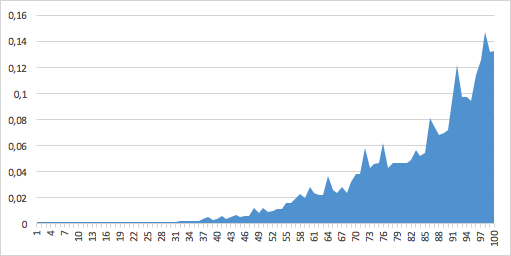
\includegraphics[width = 0.8\textwidth]{images/timeBuilder0Painter1}
    \label{fig:builder0painter1}
\end{figure}

\newpage
Warto zauważyć jak ogromne różnice w~wydajności pojawiają się, gdy wartości zmiennych sterujących rekurencją są różne. Algorytmowi pełniącemu rolę \emph{budowniczego} przy wartości zmiennej \emph{builderNestingLevel} równej $2$, dla ciągu długości $100$, podjęcie decyzji zajęło około $170$ razy więcej czasu, niż po ustawieniu wartości tej zmiennej na $1$. Wykresy \ref{fig:builder1painter1} i~\ref{fig:builder2painter1}, przedstawiają różnice w złożonościach czasowych obu rozgrywek.

\begin{figure}[tbh]
    \centering
    \caption{Liczba sekund jakiej potrzebował algorytm \emph{budowniczego} na podjęcie decyzji, przy poszczególnych długościach ciągu i konfiguracji: $\emph{setPower}=5$, $\emph{builderNestingLevel}=1$, $\emph{painterNestingLevel}=1$.}
    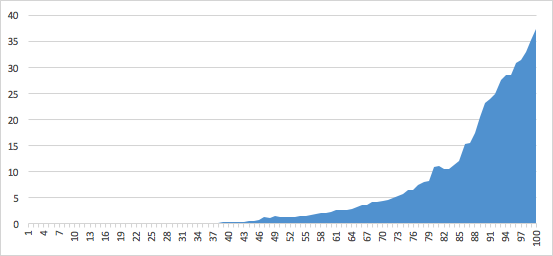
\includegraphics[width = 0.8\textwidth]{images/timeBuilder1Painter1}
    \label{fig:builder1painter1}
\end{figure}

\begin{figure}[tbh]
    \centering
    \caption{Liczba sekund jakiej potrzebował algorytm \emph{budowniczego} na podjęcie decyzji, przy poszczególnych długościach ciągu i konfiguracji: $\emph{setPower}=5$, $\emph{builderNestingLevel}=2$, $\emph{painterNestingLevel}=1$.}
    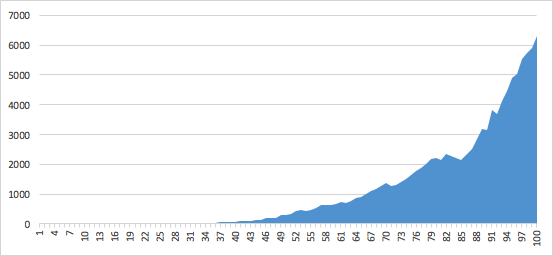
\includegraphics[width = 0.8\textwidth]{images/timeBuilder2Painter1}
    \label{fig:builder2painter1}
\end{figure}



Odrobinę inaczej wyglądają analogiczne wykresy przedstawiające złożoności algorytmów pełniących rolę \emph{malarza}. Algorytm korzystający z~rekurencji symuluje dodawanie kolejnych symboli na wyznaczonej pozycji, jeżeli jednak w~danym miejscu da się wstawić tylko jeden symbol, to algorytm przeprowadzi mniej symulacji, niż jeśli dałoby się tam wstawić pięć symboli. Dzięki tej zależności na wykresie można zauważyć, przy których ruchach \emph{malarz} jest bliski przegranej, a~przy których ma wiele dostępnych opcji. Wykres \ref{fig:painter1builder0} przedstawia czasy potrzebne algorytmowi pełniącemu rolę \emph{malarza} na podjęcie decyzji. Jak widać zachłanny algorytm działający jako \emph{budowniczy} cyklicznie redukuje liczbę opcji \emph{malarza}.



Jeśli przeanalizujemy wykres \ref{fig:painter1builder2} zauważymy, że podczas rozgrywki z algorytmem \emph{budowniczego}, który używa rekurencji, krzywe są o~wiele bardziej spiczaste, co oznacza, że dla \emph{malarza} jest to trudna rozgrywka, która ostatecznie kończy się w~$82$ ruchu. Ponownie możemy porównać ze sobą czasy jakie były potrzebne na podjęcie decyzji dla algorytmu wykorzystującego jednopoziomową rekurencję na wykresie \ref{fig:painter1builder2}, z algorytmem wykorzystującym dwupoziomową rekurencję na wykresie \ref{fig:painter2builder0}. Wykonanie ruchu, dla ciągu długości $79$ pierwszemu algorytmowi zajęło $0.061$ sekundy, natomiast temu bardziej złożonemu $17.711$ sekund. Zatem w~tym konkretnym ruchu algorytm korzystający z rekurencji głębszej o~jedno wywołanie, decydował się około $290$ razy dłużej.

\begin{figure}[tbh]
    \centering
    \caption{Liczba sekund jakiej potrzebował algorytm \emph{malarza} na podjęcie decyzji, przy poszczególnych długościach ciągu i konfiguracji: $\emph{setPower}=5$, $\emph{builderNestingLevel}=0$, \emph{painterNestingLevel}~$=1$.}
    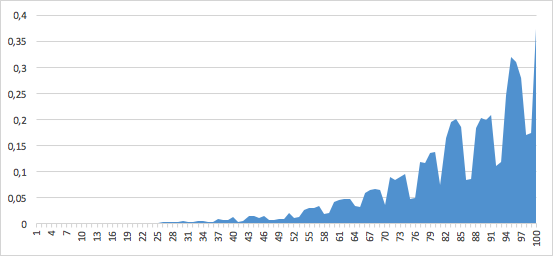
\includegraphics[width = 0.8\textwidth]{images/timePainter1Builder0}
    \label{fig:painter1builder0}
\end{figure}

\begin{figure}[tbh]
    \centering
    \caption{Liczba sekund jakiej potrzebował algorytm \emph{malarza} na podjęcie decyzji, przy poszczególnych długościach ciągu i konfiguracji: $\emph{setPower}=5$, $\emph{builderNestingLevel}=2$, \emph{painterNestingLevel}~$=1$.}
    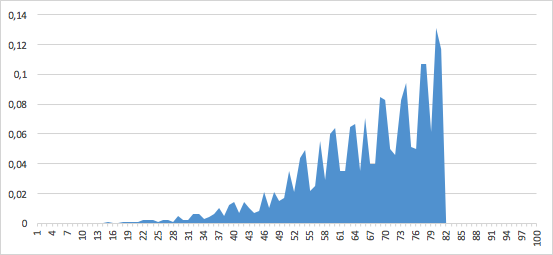
\includegraphics[width = 0.8\textwidth]{images/timePainter1Builder2}
    \label{fig:painter1builder2}
\end{figure}

\begin{figure}[tbh]
    \centering
    \caption{Liczba sekund jakiej potrzebował algorytm \emph{malarza} na podjęcie decyzji, przy poszczególnych długościach ciągu i konfiguracji: $\emph{setPower}=5$, $\emph{builderNestingLevel}=0$, \emph{painterNestingLevel}~$=2$.}
    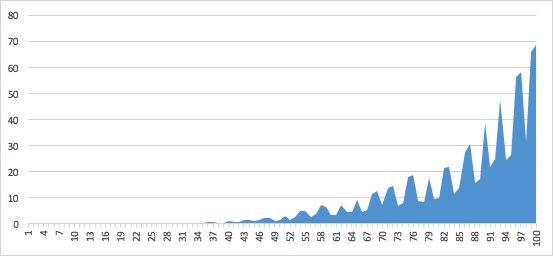
\includegraphics[width = 0.8\textwidth]{images/timePainter2Builder0}
    \label{fig:painter2builder0}
\end{figure}




\section{Porównanie zachowań algorytmu z~zagnieżdżeniami i~bez zagnieżdżeń}
Jeśli przyjrzymy się dokładnie działaniu zachłannego algorytmu wyszukiwania pozycji, to bez trudu zauważymy, że w~początkowej fazie gry, kiedy \emph{malarz} ma dużą swobodę w~wybieraniu elementów, pozycja, która jest wybierana to w~przeważającej większości ostatni indeks ciągu. Spowodowane jest to tym, że pozycje $0$ oraz $n+1$, otoczone są elementami tylko z~lewej lub prawej strony, dzięki temu \emph{malarz} ma na nich do wyboru większą gamę symboli. Na reszcie pozycji zazwyczaj dostępne jest tyle samo symboli, zwracany jest więc ostatni z~nich. Taktyka tego typu została przeze mnie nazwana \emph{taktyką iteracyjną} i~nie jest zbyt emocjonująca. Jeśli nie mamy zbyt dużej puli symboli do wyboru, to po pewnym czasie następuje wyłamanie się z~tego stylu gry. Wyłamanie pojawia się zawsze w~momencie, gdy algorytm pełniący rolę \emph{budowniczego} znajduje indeks z~mniejszą ilością możliwości. 

Przeprowadzone przeze mnie badania, przy alfabecie pięcioelementowym, zmiennych \emph{painterNestingLevel} ustawionej na $1$, i \emph{builderNestingLevel} ustawionej na $0$, wykazały, że w~przeciągu kilku kroków od pierwszego znalezienia pozycji, pod którą dostępne są dwa symbole, pojawia się pozycja pod którą dostępny jest tylko jeden symbol. Nie wykryłem natomiast korelacji, pomiędzy pierwszym wyłamaniem się z~\emph{taktyki iteracyjnej}, a~długością rozgrywki. Wykres przedstawia $10$ rozgrywek, na którym opisane są powyższe zależności.
 
\begin{figure}[tbh]
    \centering
    \caption{Stosunek pierwszego wystąpienia indeksu z dwoma dostępnymi elementami, do pojawienia się indeksu z jednym dostępnym elementem i długości rozgrywki. Użyty został pięcioelementowy alfabet, rolę \emph{budowniczego} pełnił zachłanny algorytm, a~\emph{malarza} algorytm wykorzystujący jednopoziomową rekurencję.}
    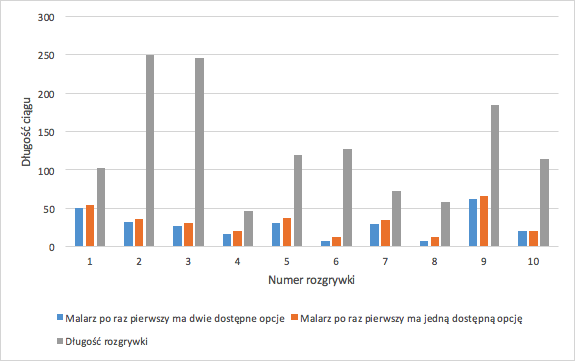
\includegraphics[width = 0.8\textwidth]{images/builder0efficiency}
    \label{fig:builder0Efficiency}
\end{figure}

Ciężko jest dopatrzyć się podobnej cykliczności w~algorytmie wykorzystującym rekurencję. Algorytm ten skupia się raczej na grupie pozycji będących obok siebie. Wykres \ref{fig:buildersPickedIndexes} przedstawia rozkład wybieranych pozycji przez oba algorytmy. Rozgrywki nie trwały dłużej niż $115$ ruchów, na rysunku można zaobserwować, że najczęściej wybierane pozycje przez algorytm rekurencyjny należały do zbioru liczb $\leq 27$. Natomiast pozycje wybierane przez algorytm zachłanny, są w~miarę równomiernie rozłożone po całej szerokości wykresu. Ponadto, mimo wyłamania się z~wcześniej wspomnianej \emph{taktyki iteracyjnej}, algorytm zachłanny w~dalszym ciągu działa cyklicznie, wybierając pozycje po zero, jeden lub pięć razy.

\begin{figure}[tbh]
    \centering
    \caption{Porównanie rozkładu wybieranych pozycji przez algorytm \emph{budowniczego} używający jednopoziomowej rekurencji oraz algorytm \emph{budowniczego} działający zachłannie.}
    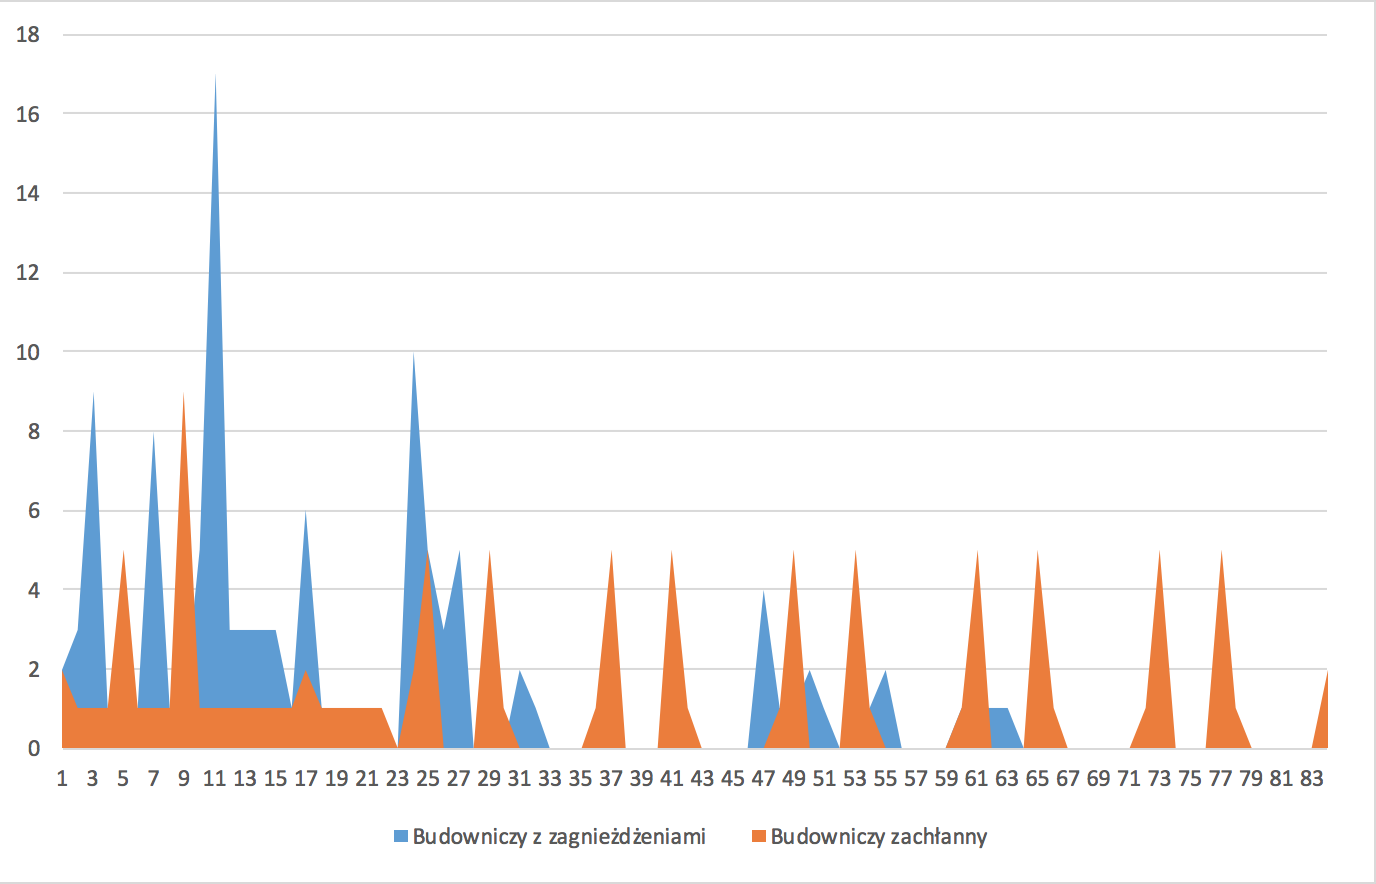
\includegraphics[width = 0.8\textwidth]{images/buildersPickedIndexes}
    \label{fig:buildersPickedIndexes}
\end{figure}

% zakończenie
\summary
Twierdzenia Axela Thue na temat sekwencji symboli okazały się doskonałą bazą do dalszych rozważań. Wykorzystali je J. Grytczuk, P. Szafruga i~M. Zmarz, tworząc grę dla dwóch graczy wykorzystującą dotychczasowe koncepcje. Podczas pisania pracy dyplomowej, postanowiłem podejść do ich pomysłu od strony programistycznej. Napisana przeze mnie aplikacja obsługuje logikę gry, wprowadza szereg funkcji ułatwiających analizę przeprowadzonych gier, a~co najważniejsze, za pomocą algorytmów jest w~stanie zasymulować rozgrywkę graczy, korzystając z wprowadzonych przeze mnie taktyk. Można dodatkowo modyfikować stworzone przeze mnie taktyki, przez zmienne konfiguracyjne, które sterują wykorzystywanym poziomem rekurencji. Ustawienie większego poziomu zagnieżdżenia skutkowało lepszymi rezultatami w~rozgrywce. Mimo to nie byłem w~stanie rzucić nowego światła na problem ilości symboli potrzebnej na dowolnie długą grę. Główną tego przyczyną jest brak zasobów sprzętowych, które pozwoliłyby na przeprowadzenie większej ilości obliczeń.

% załączniki (opcjonalnie):
\appendix

% literatura (obowiązkowo):
\bibliography{mybibfile}
\bibliographystyle{plain}



% spis tabel (jeżeli jest potrzebny):
\listoftables

% spis rysunków (jeżeli jest potrzebny):
\listoffigures

% spis listingów
\lstlistoflistings

\oswiadczenie


\end{document}
